This exercise has been completed in the attached \textit{K\_Means.ipynb} Jupyter Notebook. The most relevant bits of source code can be seen here as well:
\begin{verbatim}
data = np.loadtxt("old_faithful.csv", delimiter=',', skiprows=1)

meanData = KMeans(n_clusters=2, max_iter=30, seed=0)
meanData.fit(data)

for i in range(data.shape[0]):
    if (meanData.cluster_assignments[i] == 0):
        plt.scatter(data[i,0],data[i,1], color='blue')
    else:
        plt.scatter(data[i,0],data[i,1], color='orange')
\end{verbatim}
The 2 cluster means, calculated using the Jupyter Notebook, look as follows:
$$
\begin{matrix}
(4.29793023,80.28488372) \\
(2.09433,54.75)
\end{matrix}
$$
And the resulting images, with, with each cluster in their own colour, and the cluster means plotted as singular red dots:\\
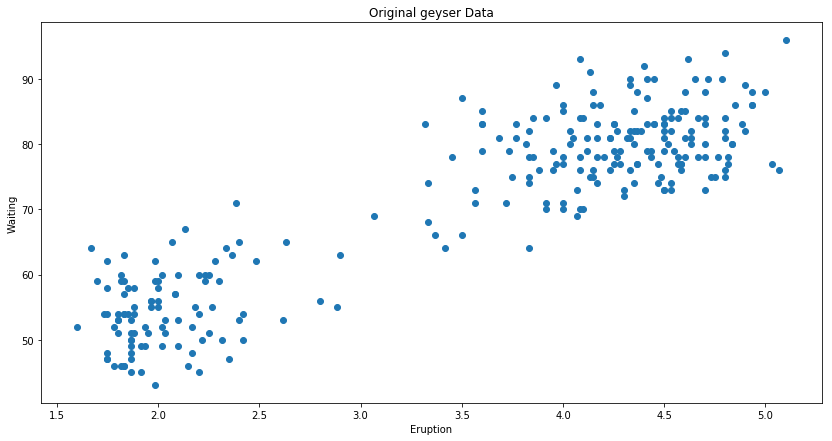
\includegraphics[width=\linewidth]{3a1.png}\\
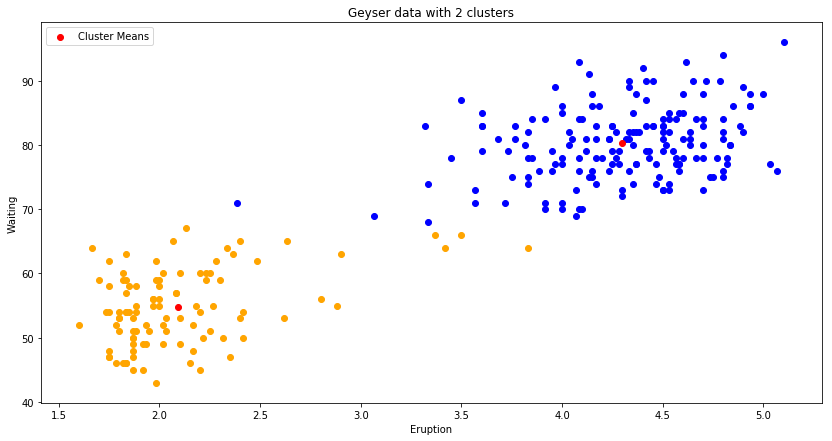
\includegraphics[width=\linewidth]{3a2.png}\\
It is relevant to note that since the "Waiting" axis is significantly larger than the "Eruption" axis, it has a large effect on where the clusters are located. This can be seen especially on the leftmost blue points, and the rightmost orange points, which a human might expect to be the other colour.